\section{Standing spin waves in Permalloy-NiO bilayers as a probe of the interfacial exchange coupling \href{https://doi.org/10.1103/PhysRevApplied.21.064044}{[\textit{Phys. Rev. Appl., 21 064044 (2024)}]}}

\subsection*{\underline{Abstract}}
The importance of ferromagnetic-antiferromagnetic (FM-AFM) bilayer dynamics, with emphasis on the interaction occurring at the interface, where the magnetic moments of the AFM can be imprinted into the FM, and the exchange bias field can affect these dynamics, is explained in this paper. Here, in this paper, they have used Permalloy (Py) and NiO (Py/NiO) hybrids, and for comparison, single Py films in the broad Py thickness range varied from a few nm to 200 nm by using static (Kerr effect) and dynamic (spin-wave) measurements along with micromagnetic simulations. Uniform precession and perpendicular standing spin waves (PSSWs, $n=1, 2)$ and a clear enhancement of the PSSW mode frequencies upon interfacing Py with NiO, both from experiments and simulations.

\hspace{1cm}The enhancement of the mode frequencies with increasing the thickness of the material, which explains its interfacial origin rooted in the exchange coupling between the FM and AFM layers. \hl{Their results suggest that PSSW detection in a ferromagnet offers a means of probing the interfacial exchange coupling with the adjacent AFM layer}. Furthermore, the controlled spatial symmetry breaking by the AFM layer enables engineering of PSSWs with different spatial profiles in the FM.

\subsection*{\underline{Introduction}}
\begin{enumerate}
    \item The focus on the investigation of ferromagnet-antiferromagnet (FM-AFM) bilayers has been concerned with the induction of uniaxial anisotropy, and recently, a thin FM layer coupled with a thick AFM layer was also studied to observe the AFM spintronics. An important factor present in both of them is the exchange coupling at the AFM-FM interface, since it's not only the shifts that we get in the static hysteresis curves, but it may also affect magnetization dynamics.
    \item Excitation of spin waves (SWs) in a FM coupled to AFM was proposed method to propagate spin excitation into the AFM \cite{jenkinsSpinWaveExcitations2020}.
    \item Recently, PSSWs have been studied in other symmetry-breaking systems like heavy metals-magnetic insulator (HM-MI) bilayers, where the frequency of the standing-wave modes experiences a shift \cite{lee2023erratum}. The effect was attributed to an additional confinement of the waves upon a local increase of the interfacial damping due to spin pumping \cite{lee2023erratum}.
    \item There are other experiments also, as per this paper, which have used PSSWs to probe coupling in FM bilayer or individual surface anisotropies on epitaxial FM layers with nonequivalent interfaces [\textcolor{red}{ref. 10-13,14}]. 

\hl{The introduction part is written in a perfect way. Please read it and get the references. Try to get the exchange length of the CoFe (B2-CsCl structure).}


    \item Lower $M_s$ is set near the top surface of our films. This translates to a lower demagnetizing field and a higher effective potential in these layers, thus enabling the pinning of the PSSW mode. [\textcolor{red}{ref. 30}].
    \item This effect might also be due to the surface oxidation typically experienced by ferromagnetic films or a magnetization symmetry breaking in the normal direction due to a capping layer.
    \item In the case of Py, the variation in the $M_s$ is the most conceivable way to induce changes in the surface pinning parameter \cite{waring2023exchange}, therefore generating magnetization symmetry breaking and allowing the excitation of PSSWs.
    \item The averaged out-of-plane (OOP) magnetization of the system was converted into the frequency domain after the use of a Fourier transform \cite{park2003imaging}. This process was repeated for each of the presented magnetic fields.
\end{enumerate}

\subsection*{\underline{Experimental Results \& Discussion}}
\begin{enumerate}[A.]
    \item \underline{Static Characterization of the Py and Py/NiO films:}
    \begin{enumerate}[1.]
        \item Static MOKE reveals the clear enhancement of the ferromagnetic films upon the addition of NiO. As expected, there is an exchange bias in the FM/AFM layer.
        \item Experimentally, it has been proved that this phenomenon will suppress once the thickness of the FM layer becomes large enough, which can be attributed to the reduced effect of the interface exchange coupling strength relative to the overall magnetization of the film.
        \item They have also observed the shift in the hysteresis loops from a field-centered position, which clearly indicates the presence of an exchange bias field in Py/NiO.
        \item There is also a reduction in the exchange bias field as the Py layer becomes thicker, once again, an effect related to the reduced influence on the overall film magnetization. \hl{Quantifiable exchange coupling within our AFM-FM films}
    \end{enumerate}
    \item \underline{Effect of NiO on the frequency of the observed standing waves}
    \begin{enumerate}[1.]
        \item After doing the VNA-FMR, they have observed a uniform FMR mode, characteristic of the FM layers in the case of both Py and Py/NiO.
        \item The spin-wave modes are identified as exchange-dominated thickness-dependent modes related to PSSWs in our films \cite{dabrowski2021canted}.
        \item The existence of different PSSW modes with the thickness of the films is also observed. 
        \item In this system, the PSSW modes were shifted to higher frequencies, replacing the standing spin-wave modes. The frequency shift decreases with the enhancement of the thickness of the Py layer.
        \item This suggests that there is a direct relation between the magnitude of the magnetic moments in the film as the FM layer grows thicker and the frequency shift of the PSSW modes experienced when the NiO layer is added.
        \item Generally, FMR mode is independent of the thickness; however, in this case, when the thickness is increased, they have observed the frequency shift in the same direction for all of the pairs of samples.
        \item The frequency shift experienced by our films is a direct consequence of the Py magnetic moments pinning at the interface due to the exchange bias. The absence of free spins results in an additional confinement of the PSSWs.
        \item There is the confinement of the PSSW modes when the thickness is reduced to 2 nm, and it is supported by the experiments done on thin films.
        \item The saturation magnetization remained consistent at all thicknesses in the case of Py/NiO.
        \item The anisotropy field progresses similarly to the exchange bias and coercive fields extracted from the static hysteresis loops. This is expected since the exchange bias of the films has less influence on the overall magnetization as the film thickness increases.
        \item There is an increase of Gilbert damping (almost an order of magnitude for smaller Py samples) for Py/NiO. This might be the influence of spin pumping to AFM \cite{wang2020spin} and exchange bias at the interface, freezing the magnetic moments of the Py and preventing larger precessions.
        \begin{figure}[ht]
            \centering
            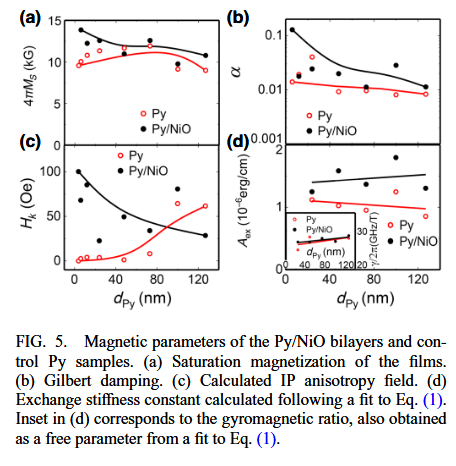
\includegraphics[width=0.65\linewidth]{Images/PSSW_01.png}
            \caption{\textit{Figure from the paper, important one}}
            \label{fig:PSSW_pp1_01}
        \end{figure}
    \end{enumerate}
\end{enumerate}
\subsection*{\underline{Numerical Results of PSSW presence of Py films}}
\begin{enumerate}[1.]
        \item The thickness of the Py films used in the simulation (done by using Mumax$^3$) ranges from 20 nm - 200 nm.
        \item The films are thick enough to accurately resolve the PSSW modes and to observed their possible shifts in the frequency when the interaction with the AFM is introduced.
        \item The surface magnetization gradient caused by a possible oxidation and/or capping, they aim to manipulate the interface pinning parameter, which strongly affects the spin configuration of the PSSW modes across the film \cite{waring2023exchange}.
        \item Not taken in account the surface anisotropies.
        \item Weaker modes above 30 GHz are not observed experimentally in our system due to the strong losses experienced at high frequencies.
        \item In the case of simulation, the detected nodes, $n>0$ are proportional to $1$/$d^2_{Py}$. This agrees with the reports on PSSWs in other FM films.
        \item The frequency of the bulk FMR remains constant when the thickness of the film is increased. Eventually, two modes combine at $d_{Py}< 110$ nm.
\end{enumerate}
\begin{enumerate}[A.]
    \item \underline{Simulating the Py/NiO interface. Optimization of the Uniaxial anisotropy}\\
    The simulations of magnetization dynamics in the AFM-FM bilayer were performed by introducing an extra layer in the system as an uncompensated AFM. This leads to uncompensated spins at the interface, which lead to an exchange bias between FM and AFM.
    \item \underline{Hybrid modes and effect of the interaction with the antiferromagnet}
    \begin{enumerate}[1.]
        \item In both micromagnetics and Atomistic simulations, AFM sublattices are used to model the system \cite{jenkinsAtomisticOriginAthermal2021,jenkinsAtomisticOriginExchange2020}.
        \item Shift in the frequency of the modes, especially in the experimentally observed first-order PSSW $(n=1)$, is also present in all of the performed simulations featuring an AFM-FM interface.
        \item The uniaxial anisotropy at the interface has a direct influence on the frequency of the PSSWs. As given in the diagram, uniaxial anisotropy induced by the AFM leads to higher-frequency modes.
        \item The frequency of the modes can be further enhanced by introducing a local in-plane exchange bias field in the bottom layer of the order of $H_{eb}=1$ kOe. 
    \end{enumerate}
    \item \underline{Conclusion}
    \begin{enumerate}[1.]
        \item They have detected both perpendicular PSSWs spin waves and quasiuniform modes and found that in sufficiently thick Py films both exhibit a clear frequency shift when Py is exchange coupled to NiO.
    \end{enumerate}
\end{enumerate}